\begin{figure}[!htbp]
\centering
{\small
\textcolor{green!60!black}{Top silicon}\quad
\textcolor{red}{Gate oxide}\quad
\textcolor{blue}{BOX}\quad
\textcolor{cyan!60!black}{Silicon substrate}}\par\smallskip
{\small (a) Whole one-dimensional material stack}\par
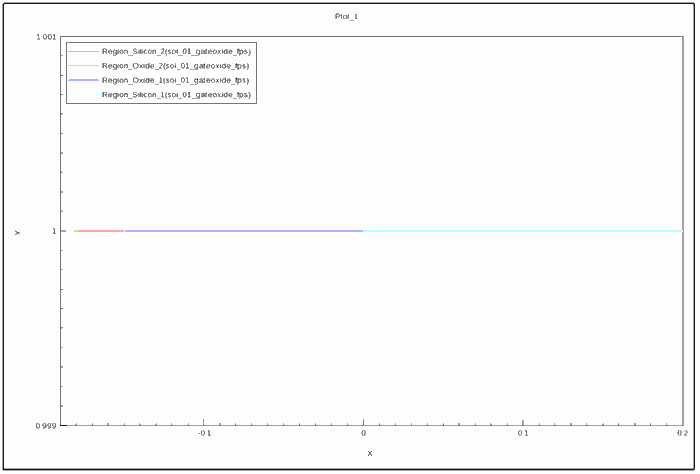
\includegraphics[
  width=.96\linewidth,
  trim=0bp 5bp 0bp 105bp,clip
]{figures/01_gateoxide_full_svisual.png}
\par\smallskip
{\small (b) Zoom at the gate-oxide/silicon interface}\par
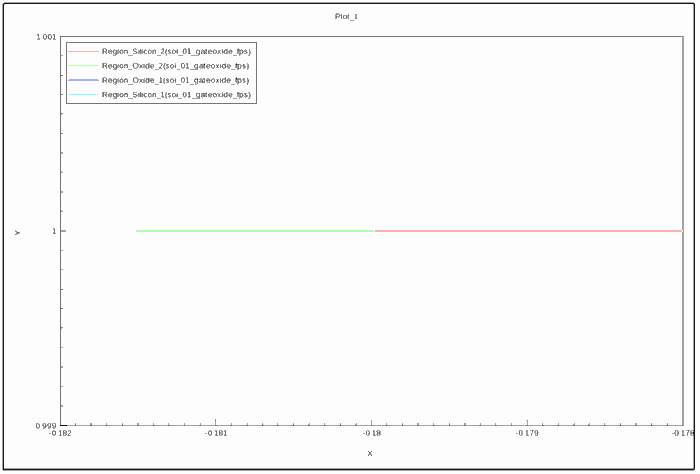
\includegraphics[
  width=.96\linewidth,
  trim=0bp 5bp 0bp 105bp,clip
]{figures/01_gateoxide_zoom_svisual.png}
\caption{Original SVisual screenshots from
\texttt{soi\_01\_gateoxide\_fps.tdr}, cropped only to remove
empty upper plotting space while keeping the original aspect
ratio and depth axes. The colored lines at $Y=1$ are
region-membership indicators, not device-current traces.
The gate oxide is \texttt{Region\_Oxide\_2} (green) and
the underlying film is \texttt{Region\_Silicon\_2} (red).
The oxide thickness of 1.532\,nm comes from the original
SProcess region-interface coordinates, not screenshot pixels;
its source-derived physical-depth diagram appears in
Fig.~\ref{fig:gate_oxide_material_profile}.}
\label{fig:part1_gateoxide_svisual_actual}
\end{figure}
